\documentclass[12pt,journal,compsoc]{IEEEtran}

%%% Packages
\usepackage{array}
\usepackage{amsmath}
\usepackage{caption}
\usepackage{fancyhdr}
\usepackage{graphicx}
\usepackage{float}
\usepackage[LGRgreek]{mathastext}
\usepackage{lipsum}
\usepackage{multirow}
\usepackage{subfigure}
\usepackage{url}
\usepackage{varwidth,xcolor}

%%% Document
\begin{document}

% Title
\title{Comparison of Denoising Algorithms}
\author{Paola Ardon, Jose Bernal, Rodrigo Daudt, Seperh Mohaimanian, \`Eric Pairet, Armine Vardazaryan
\vspace{0.2cm} \\
        \small{Department of Electrical Engineering, University of Burgundy, France \\
        %$^1\,$ \textit{ardonp@hotmail.com} \\
		%$^2\,$ \textit{jose.bernal@correounivalle.edu.co} \\
        %$^3\,$ \textit{rcdaudt@gmail.com} \\
		%$^4\,$ \textit{Voidminded@gmail.com} \\
        $^*\,$ \textit{eric.pairet@u-bourgogne.com} \\
        %$^6\,$ \textit{arminevardazaryan@gmail.com}
        }}
        
% Paper header
\markboth{KSVD} {KSVD}
\setlength\headheight{26pt}

% Abstract
\IEEEtitleabstractindextext{
\begin{abstract}
Abstract...
\end{abstract}

% Key words
\begin{IEEEkeywords}
Key words...
\end{IEEEkeywords}}

% Make the title area
\maketitle




% Sections
%\section{Introduction}

Nowadays, one of the main challenges of medicine and engineering is to develop tools for supporting the medical diagnosis. According to the World Health Organization (WHO), about 15\% of the population's deaths between 2010 and 2020 will be caused by Non-Communicating Diseases (NCD), such as cardiovascular diseases, diabetes, cancer and chronic respiratory diseases~\cite{who}. Thus, the target of this medical tools is to detect timely these diseases such that they can be cured or controlled.  %%Need to build a bridge between this parag. and the next one.

In particular, diabetes detection has been carried out through Retinopathy Image Analysis (RIA). Fundus cameras, scanning lasers, angiography, and, more recently, Optical Coherence Tomography (OCT) are some techniques to acquire retinopathy images. It is important to be aware that these images may be corrupted by noise during the acquisition process. This is due to limitations of sensor capabilities and characteristics, transmission issues, among other facts. As a result, low-quality images, which may not be suitable for medical analysis, are obtained. 

There are different types of noise arising during the acquisition process and also varied techniques trying to overcome them. The criteria for deciding which algorithm to use usually depends on the specific features and constraints of the scenario. Ideally, the type and level of noise are known beforehand. However, most of the time, the case is the opposite and estimation and characterisation of the noise are required. Under this perspective, there are two questions that should be answered before deciding how to address the situation:
(1) Is there any a priori knowledge about the situation? The selection of denoising techniques is fundamental and it can be guided by knowledge of the data to process. Selecting wrongly an algorithm may distort the image instead of improving its quality. (2) What is the goal? There are different approaches for image denoising, but some of them are not suitable for some applications. For instance, Weiner filter is used for removing noise in the sense of Mean Square Error (MSE) but it is not desired for applications in which the visual perception is the target. Having this in mind, there is no algorithm capable of denoising every image and, thus,  expectations should be clear before addressing the problem.

In this paper, an evaluation of different state-of-the-art algorithms for noise removal is presented. The paper is organized as follows. Considered algorithms are described and examined in Section \ref{sc:state-of-the-art}. Synthetic and retinopathy datasets for performing the experimental validation are introduced in Section \ref{sc:experimental-validation}. The considered algorithms are tested following the experimental validation and the final results are analysed in Section \ref{sc:results}. Finally, some final remarks and future work are presented in Section \ref{sc:final-remarks}. 
%\section{Denoising Algorithms} \label{sc:state-of-the-art}
%%We can add kind of intro to this section
In the following sections, we discussed the idea behind some traditional and state-of-the-art denoising algorithms as well as their advantages and disadvantages.

\subsection{Mean filter}

Given a noisy image $g$, the restored value on the denoised image $\hat{f}$ at the position $(x, y)$ corresponds to the average of the neighbourhood $N$ (See Eq. \ref{eq:mean-filter}).

\begin{equation}
	\hat{f}(x, y) = \frac{1}{M\cdot N}\sum_{(u, v) \in N(x, y)}{g(x, y)}.
    \label{eq:mean-filter}
\end{equation}

This process acts on the supposition that the noise is concentrated on the upper part of the frequency spectrum. This approach is able to remove pixels which are not representative in the considered neighborhood and also reduce the noise by blurring the image. Thus, high frequencies are lost during the process.

This is the simplest denoising method and is not very effective. Denoising through mean filter simply applies a linear transformation to the image (a convolution with a smoothing kernel), and it makes no attempt to interpret the information in the image and use it in the denoising process.

The main drawbacks of this method is that is sensible to outliers and that it blurs the processed image.

\subsection{Median filter}

Median filter is a spatial filter based on order-statistics. It replaces the value at each position with the 50th percentile of the neighborhood (See Eq. \ref{eq:median-filter}). 

\begin{equation}
	\hat{f}(x, y) = {median}_{\substack{(u, v) \in N(x, y)}}{g(x, y)}.
    \label{eq:median-filter}
\end{equation}

Unlike mean filter, median filter is able to detect outliers of a neighborhood and remove them with a smaller impact on the higher frequencies. For the same reason, this filter is well-known for denoising images affected by salt-and-pepper noise. 

%The main drawback of this method is its computational complexity for large groups of data. % What? No!

\subsection{Filtering by use of local statistics (LS filter)}

Digital Image enhancement by using local statistics is a computational technique that involves contrast and noise filtering on two-dimensional arrays based on their local mean and variance. One of the greatest advantages of this type of algorithms is that they are non-recursive and each pixel is processed independently. As a consequence this approach has a great advantage when is used in real time image processing.

This algorithm was developed to overcome the greatest problem of early techniques in image processing, the computation of the image transformation. Usually, the Fourier or Walsh transform does not represent a big setback for one dimensional data array, however it was very time consuming for a two dimensional array. As a result, these early techniques were proved not to be suitable for real time image processing applications.

The assumption of the algorithm based on local statistics is that the sample mean and variance of a pixel is equal to the local mean and variance of all the pixels within a fixed range. For example, in the additive noise filtering case, the variance is calculated as the difference variance of the noise in the corrupted image and the noise itself, the same method is used for multiplicative noise.
This simple approach has been pointed as to lack mathematical elegance and sophistication, compared to other techniques, however the results indicate it is a very effective tool for contrast stretching and noise filtering of images.

Let $x_{ij}$ be the brightness of the pixel $(i,j)$ in a two dimensional $N\times N$ image. The local mean and variance are then calculated over a $(2n+1) \times (2m+1)$ window. The local mean is defined as:

\begin{equation}
    \mu_{ij}=\dfrac{1}{(2n+1)(2m+1)}\sum_{k=i-n}^{n+i}\sum_{l=j-m}^{m+j}{x_{kl}},
    \label{eq:ls_filter_1}
\end{equation}

and the local variance is:

\begin{equation}
    v_{j} =\dfrac{1}{(2n+1)(2m+1)} \sum_{k=i-n}^{i+m}\sum_{l=j-m}^{j+m} (x_{kl} - \mu_{ij} )^2.
    \label{eq:ls_filter_2}
\end{equation}

From these equations it is not hard to extend the algorithm to deal with images corrupted by additive or multiplicative noise or even both. A noisy corrupted image is described as: 

\begin{equation}
z_{ij} = x_{ij}*u_{ij} + w_{ij}.
    \label{eq:ls_filter_3}
\end{equation}

Where the mean and variance are calculated as:

\begin{equation}
    E[(u_{ij} - \vec{u_{ij}})( u_{kl} -\vec{u_{kl}})] = \sigma^2*\delta_{ik}*\delta_{jl}.
    \label{eq:ls_filter_4}
\end{equation}

From the structure of the algorithm, it is easy to see that the principal computational load relays on the calculation of the local mean and variance of the image. To make the calculations faster, an improvement to the algorithm is proposed where the image is partitioned in square sub regions over which the local variance and mean are calculated. Further, the local mean and variance of a pixel are approximated by the use of two dimensional interpolation formulas. This improvement seems to be promising and perfectly suitable for real time -parallel image processing.

\subsection{Hard and soft thresholding in wavelet domain (wavelet filter)}
Wavelet transform is a signal processing technique for cases when frequency varies over time. For certain classes of signals and images, wavelet analysis provides more precise information about signal data than other signal analysis techniques.

The wavelet transform is used extensively in signal de-noising. The usual way to de-noise signals in wavelet domain is to first transform the signal into wavelet domain, apply hard or soft thresholding and then transform back. 

Hard thresholding is a noise suppression method, that applies the following transformation to the empirical wavelet coefficients:

\begin{equation}
    F(x)=x\cdot I(|x|>t),
    \label{eq:wavelet_1}
\end{equation}

where $t$ is a threshold value. For de-noising to perform adequately, $t$ must be chosen carefully.

The theoretically optimal value for $t$ is $t=\sqrt{2\sigma^{2}log(n)/n}$, where $\sigma^{2}$is the variance of the noise and $n$ is the length of input data. In practice, usually, a smaller value is usually used ~\cite{thresholding}.

Soft thresholding, just like hard thresholding, incorporates a transformation of the empirical wavelet coefficients. The only difference is the chosen nonlinear transformation:

\begin{equation}
    S(x)=sign(x)(|x|-t)\cdot I(|x|>t),
    \label{eq:wavelet_2}
\end{equation}

where, again, $t$ is the threshold value.

However, when the signal contains discontinuities, the denoising will also result in artifacts: pseudo-Gibbs phenomena, when the signal is alternatingly overshooting or undershooting its level. These artifacts depend on the precise alignment between the signal and the basis elements, therefore depend both on wavelets and the input data. 

A solution was proposed in "Translation-Invariant De-Noising"~\cite{wavelet}, where Coifman and Donoho present an algorithm to minimize the effects of this phenomenon. They propose to shift the signal prior to thresholding, then shift the signal back. This can be done for both time and frequency shifting. For the case of a time-shift, let $S_{h}$ denote the circulant shift by $h$: $(S_{h}x)_{t}=x_{(t+h)}, $where $x_{t}\in0\leq t\leq n$ is the given signal. A frequency shift by $\xi$ can be represented as follows: $(M_{\xi}x)_{t}=e^{i\xi t}x_{t}$, where $M_{\xi}$ is the modulation. To incorporate the shifting into the denoising scheme, signal is first shifted, de-noised then unshifted. A better way is to average the result of this process using a range of shifts.

Because there is no single 'right' choice for the shift parameters $h$ and $\xi$ that will yield the best result for all signals, the authors use a technique called cycle-spinning, where the wavelet de-noising is averaged over all $n$ circulant shifts, without restraining the value to a range. This technique is translation invariant and requires only $n\log(n)$ time.

\subsection{Subspace}
Synthetic aperture radar (SAR) imaging technique is a popular technique for remote sensing and monitoring applications because of its usability under various weather conditions and its ability to provide high-resolution imagery. A SAR image is generated by sending electromagnetic waves from a moving platform, space borne or airborne, toward the target surface and by coherently processing the returned backscattered signals from multiple distributed targets. However, the coherent processing causes speckle effect and gives SAR images its noisy appearance. Speckle presence appears as granular noise which reduces the image resolution and may hamper the operation of image interpretation and analysis.

\subsubsection{Adaptive spatial-domain filters}
The assumptions made in implementing these filters are as follows:

\begin{itemize}
	\item The SAR speckle is modeled as a multiplicative noise
	\item The noise and signal are statistically independent
	\item The sample mean and variance of a pixel are equal to its local mean and local variance computed within a window centered on the pixel of interest
\end{itemize}

The Lee and Kuan filters have similar formation but differ in signal model assumptions and derivation. The  filters achieve a balance between averaging in homogeneous regions and a strict all-pass (identity) filter in edge contained regions. 

The Frost filter attempts to strike a balance between averaging and identity filter by forming an exponential-shaped filter kernel that can adaptively vary from an average filter to an identity filter. At low coefficient variation, the filter is more average-like and, at high coefficient variation, the filter attempts to preserve sharp features by retaining its original pixel value.

The enhanced Lee and Frost filter uses three variations of coefficient values, namely, low, intermediate, and high, to divide an image into homogeneous regions,
heterogeneous regions, and isolated point target regions, respectively. The filter outputs a local mean at homogeneous regions and retains the original pixel at points of high activity.

\subsubsection*{Disadvantages}
\begin{itemize}
	\item Fail to maintain the mean value, particularly if the number of look of the original
SAR data is small.
	\item The highly reflective point targets are blurred.
	\item The highly reflective point targets are blurred.
\end{itemize}

\subsubsection{Wavelet transform}
An outcome of wavelet theory, denoising in the discrete wavelet transform (DWT) domain may be stated as a thresholding of DWT coefficients of the noisy image. The log-transformed noisy image is either adaptively thresholded or empirically shrunk in an adaptive fashion has been utilized. The major drawbacks of such approach are the backscatter mean preservation in homogeneous areas, sharpness preservation, and
ringing impairments. To overcome these deficiencies, Argenti proposed a minimum-mean-square error filtering performed in the decimated wavelet domain by means of
an adaptive rescaling of the detail coefficients and the local space-varying signal, where the noise statistics are estimated in the wavelet domain. Using statistical modeling of wavelet coefficients, Ranjani et al. proposed a speckle suppression technique using dual-tree wavelet transform by putting into consideration the significant dependences of the wavelet coefficients across different scales. The
interscale dependence of the wavelet coefficients in each sub-band is modeled using bivariate Cauchy probability density function (pdf).

\subsubsection{Subspace-based technique}
To decompose the vector space of the noisy image into a signal-plus-noise subspace and the noise subspace. The noise removal is achieved by nulling the noise subspace
and controlling the noise distribution in the signal subspace. For white noise, the subspace decomposition can theoretically be performed by applying the Karhunen-Loeve transform (KLT) to the noisy image. Linear estimator of the clean image is performed by minimizing image distortion while maintaining the residual noise energy below some given threshold.

\subsubsection*{For colored noise}
\begin{enumerate}
\item A prewhitening approach prior to KLT transform.
\item A generalized subspace for simultaneous diagonalization of the clean and
noise covariance matrices.
\end{enumerate}

\subsubsection*{Problem}
The fundamental signal and noise model for subspace methods is additive noise uncorrelated with the signal. In SAR images, the noise is multiplicative in nature.

\subsubsection*{Solution}
\begin{itemize}
	\item A homomorphic framework takes advantage of logarithmic transformation in order to convert multiplicative noise into additive noise.
	\item But this nonlinear operation totally changes the statistics of SAR images and
induces bias in their mean values. For the purpose of radiometric preservation, the biased mean needs to be corrected, along with antilog operation.
\end{itemize}

\subsubsection{Statistical modeling of speckle noise in SAR images}
With homogeneous targets and weakly textured areas in SAR images, the speckle noise is fully developed, and the multiplicative model is used to describe it. Since
most available image denoising techniques were developed for additive white Gaussian noise (AWGN), it is necessary in case of a fully developed speckle noise to apply a logarithmic transform to the multiplicative model in order to convert it into additive. The process involves applying logarithmic transform prior to the denoising technique and then exponentially transforming the output to obtain the despeckled image. As a nonlinear operation, the logarithmic transform totally changes the statistics of SAR images, so the original speckle statistics cannot directly be used with
the log-transformed images. In this section, the pdf, mean, and standard deviation values of the log-transformed speckle noise are briefly discussed. The purpose is to correct the biased mean for radiometric preservation. SAR images are usually available in two formats: intensity and amplitude:

\subsubsection*{Intensity Format}
\begin{equation}
	G = W\times N
    \label{eq:subspace-intensity-format}
\end{equation}

$G$ denotes the SAR image intensity, $W$ is the backscattering coefficients. Applying the logarithmic function to both sides of \ref{eq:subspace-intensity-format}, we get
\begin{equation}
	\log(G)=\log(W)+\log(N)
\end{equation}
Finally, a table of mean and standard deviation of speckle noise in linear and logarithmic scales is constructed as follow
\begin{table}
\centering
\caption{Mean and standard deviation of speckle noise}
\begin{tabular}{|c|c|c|c|c|}
\hline
\textbf{L} & \textbf{$\overline{N_{l}}$} & \textbf{$\overline{v_{N_{l}}}$}  &  \textbf{$\overline{N_{l}}(dB)$} & \textbf{$\overline{v_{N_{l}}}(dB)$} \\ \hline
1  & $\overline{N_{l}}$ & $\overline{N_{l}}$ & 10 $\log\overline{N_{l}} -2.507$ & $5,570$ \\ \hline
2  & $\overline{N_{l}}$ & $\overline{N_{l}}\sqrt{2}$ & $10 \log \overline{N_{l}} -1.174$ & $3,488$ \\ \hline
4  & $\overline{N_{l}}$ & $\overline{N_{l}}\sqrt{2}$ & $10 \log \overline{N_{l}} -0.556$ & $2,314$ \\ \hline
10 & $\overline{N_{l}}$ & $\overline{N_{l}}\sqrt{2}$ & $10 \log \overline{N_{l}} -0.221$ & $1,408$ \\ \hline
20 & $\overline{N_{l}}$ & $\overline{N_{l}}\sqrt{2}$ & $10 \log \overline{N_{l}} -0.109 $ & $0,983$ \\ \hline
\end{tabular}
\label{tab:subspace-mean-deviation-speckle-noise}
\end{table}

\subsubsection*{Amplitude Format}
If Eq. \ref{eq:subspace-intensity-format} is in amplitude format and $L = 1$, then the pdf of N obeys the Rayleigh pdf. For
$L > 1$ amplitude image, different techniques are used to obtain a closed analytical
form for the pdf. Among these techniques, there are histogram estimation technique
and approximation method using Edgeworth expansion.

\subsubsection{Subspace-based spatial domain constraint approach (SDC)}
The noise here is assumed to be AWGN, uncorrected with the signal, after using a weighting scheme. Eventually, the implementation of Signal Subspace Approach for Uncorrelated Speckle Noise is as follow:
\begin{enumerate}
\item Apply the homomorphic transformation to the noisy image
\begin{equation}
	Y_1=\log(G)
\end{equation}
\item Estimate the noise variance $v^{2}$
\item Compute the dimension of signal subspace $r$.
\item Using the estimated $r$ in step 3, apply eigen decomposition on RYl ; then, extract
the basis vectors of signal subspace $U_1$ and their related eigenvalues
\begin{equation}
	\triangle _X^i = \triangle _y^i-v_n^2
\end{equation}
\item After estimating $\mu$, the optimum linear estimator is computed.
\begin{equation}
	H_{SDC}= U_{1}\triangle _{X_1}(\triangle _{X_1}+\mu v_n^2I)^{-1}U_1^T
\end{equation}
\item Compute the clean image
\begin{equation}
	\hat{X_{l}}=H_{SDC}Y_{l.|}
\end{equation}
\item Reverse the homomorphic effect by taking the exponential of $X_l$ as follows:
\begin{equation}
\hat{X_{l}}=10^{\hat{X_{l}}}.|
\end{equation}
\item Apply bias adjustment according to Table \ref{tab:subspace-mean-deviation-speckle-noise}.
\end{enumerate}

\subsection{BMxD}
BM3D is an image denoising strategy which uses block matching and collaborative filtering in 3D domain.

The aim of bloc matching is to stack similar 2D image fragments ("blocks"), in 3D arrays which are called "groups". Similarities are computed between candidate fragments at different spatial locations and each reference fragment. The groups are disjoints, so some blocks can be stacked in multiple groups. These groups have a "diameter" which is the maximum number of blocks inside.

After getting the groups by block matching, a collaborative filtering is applied, which includes : 3D transformation, shrinkage of the transform spectrum, and inverse 3D transform. Different 3D transformations can be applied according to the type of noise, or it can be decomposed in 2D transform followed by 1D transform.

The last process used is the aggregation. Because the groups are disjoints, multiple estimates are given for some blocks so they will overlap. In order to aggregate them, the blocks are awarded with weights. For each final pixel, the block pixels corresponding are averaged with their given weights.

The algorithm is divided in two steps. The first one consists in applying block matching and collaborative filtering on the noisy image. The shrinkage of the coefficients of the 3D group is realised for this first step with an Hard-Thresholding filter. The basic estimate got from the first step helps to improves an other block matching in the second step. Collaborative filtering is applied once again on these new obtained blocks and the shrinkage is now realised by a Wiener filter, which attenuates the frequencies using the signal to noise ratio. The final estimate is therefore obtained, what corresponds to the denoised image.

Multiple parameters can be tuned in order to choose between a faster or more accurate algorithm, like : block size, group diameter, step between reference blocks and search area.

This method improves the non-local mean filter method in using 3D transform instead of 1D. Thanks to the filtering in transform domain applied on the already process groups, the method shows good preservations of uniform areas, smooth intensity transitions, textures, repeating patterns and sharp edges. The main advantages of this approach is the non-locality and the collaborative filtering

\subsection{K-SVD} \label{sc:description-ksvd}
This method of de-noising is based on sparse and redundant representations over trained dictionaries. In ~\cite{ksvd} the authors propose two possible implementations: with a dictionary pre-trained with high quality images, or with training a new dictionary using the corrupted. The algorithm minimizes the number of components $||\alpha||_{0}, $ while the error $||D\alpha-X||_{2}$ is bounded, where $D$ is the used dictionary, $X$ is the input image image and $\alpha$ is a vector that represents the columns of dictionary $D$ needed to reconstruct the image $X$. $X$ is processed in small patches of $\sqrt{n}$ x $\sqrt{n}$. The used dictionary must be based on the Sparseland model: The Sparseland model can be represented with the triplet $(\epsilon,L,D)$, where $\epsilon$ is the upper limit for the sum of the square differences between the input image and its denoised version, $D$ is the used overcomplete dictionary, and $L$ is the maximum number of non-zero elements in $\alpha$. It is required that the corrupted image in this algorithm belong to the Sparseland model. That means that all $\sqrt{n}$ x $\sqrt{n}$ patches in the image can be represented through columns of the matrix $D$.

The Sparseland dictionary $D$ can be iteratively trained using image patches($Z$) of good quality, each of size $\sqrt{n}$ x $\sqrt{n}$. At each iteration, $D$ can be found through minimizing the following expression:

\begin{equation}
    \epsilon(D,\{a_{j}\}_{j=1}^{M})=\displaystyle \sum_{j=1}^{M}[\mu_{j}||\alpha||_{0}+||D\alpha_{j}-z_{j}||_{2}^{2}],
    \label{eq:ksvd_1}
\end{equation}

where $\mu$ is chosen implicitly. 

The next step, then, is to use $D$ to compute a set of near-optimal vectors $\alpha$,

\begin{equation}
    \hat{\alpha}_{ij}=arg \displaystyle\min_{\alpha} \mu_{ij}||\alpha||_{0}+||D\alpha-x_{ij}||_{2}^{2}.
    \label{eq:ksvd_2}
\end{equation}

This process guarantees a decreasing error after each iteration. 

Alternately, patches from the corrupted image can be used for training the dictionary $D$, as K-SVD dictionary learning process has a noise rejection capability.

In this case, at first, $D$ is assumed to be known. We can begin the process using a pre-trained dictionary or using any overcomplete dictionary such as an overcomplete DCT dictionary. The problem is then defined as

\begin{equation}
	\begin{split}
    		\{\hat{D},\hat{\alpha}_{ij},\hat{X}\} = &arg \displaystyle\min_{\hat{D},\hat{\alpha}_{ij},\hat{X}}\,\lambda||X-Y||_{2}^{2}\\&+\displaystyle \sum_{ij}\mu_{j}||\alpha||_{0}+\displaystyle \sum_{ij}[||D\alpha_{ij}-R_{ij}X||_{2}^{2}],
	\end{split}
    \label{eq:ksvd_3}
\end{equation}

where $R$ is a matrix that extracts all the (i,j) patches from the image in the Sparseland format and $Y$ is the corrupted image.

First, $D$ and $X$ are assumed fixed, which permits to compute $\hat{\alpha}_{ij}$. Then, given $\hat{\alpha}_{ij}$, the dictionary $D$ can be recomputed using K-SVD. After that, using both $D$ and $\alpha$, an output image $X$ can be computed:

\begin{equation}
    \hat{X}=arg\displaystyle\min_{x}\,\lambda||X-Y||_{2}^{2}+\displaystyle \sum_{ij}[||D\hat{\alpha}_{ij}-R_{ij}X||_{2}^{2}].
    \label{eq:ksvd_4}
\end{equation}

But because the new $X$ will have a different level of noise, and that value is used in preceding steps, a few more iterations of this process are performed.

Summarizing, this denoising method is based on local operations and involves a sparse decomposition of the image blocks, using a dictionary. The dictionary is trained on patches of a noisy or a high-quality image.

\subsection{NLM}

Non local means (NL-means) algorithm for image denoising in ~\cite{nlm} is based on a non-local averaging of all pixels in the image. The main difference of the NL-means algorithm compared to local filters or frequency domain filters is the systematic use of all possible self-predictions the image can provide, a principle used also in ~\cite{texture}. There are many different methods for denoising image with common technique of averaging. This averaging may be performed locally: the Gaussian smoothing model ~\cite{gabor}, the anisotropic filtering ~\cite{anisotropic} and the neighborhood filtering ~\cite{neighbour}, by the calculus of variations: the Total Variation minimization ~\cite{variation}, or in the frequency domain: the empirical Wiener filters ~\cite{neighbour} and wavelet thresholding methods~\cite{soft}. 

Non local means algorithm is based on the following equation:

\begin{equation}
	\begin{split}
		NL&[u](x)=\\
        &\frac{1}{C(x)}\int_{\Omega} e^{-\frac{(G_a*\mid u(x+.)-u(y+.)\mid ^2(o))}{h^2}}u(y)dy,
	\end{split}
\end{equation}
where $x \epsilon\, \in\,  \Omega$,
\begin{equation}
	\begin{split}
	    C(x)&= \\
        &\int_{\Omega} e^{-\frac{(G_a*\mid u(x+.)-u(y+.)\mid ^2(o))}{h^2}}u(y)dy
    \end{split}
\end{equation}
is a normalizing constant, $h$ is the filtering parameter and $G_a$ is a Gaussian kernel. The new value of a pixel $x$ is defined as the mean of all the pixels in the image whose neighborhood is similar to the neighborhood of $x$.

\begin{equation}
	NL[v](i)=\sum_{j\space\epsilon\space I}{w(i,j)\cdot v(i,j)},
\end{equation}

where $v= \{v(i)  \mid  i \in I \}$ represents all the pixels in an Image and the weights for each pixel depend on the similarity between the two pixels I and j. The weights {w(i,j)}, depend on the similarity between two pixels I and j under the conditions: $0 < w(i,j)< 1,\,\sum_{j}{w(i,j)}=1$.

The similarity between two pixels i,j is determined by the similarity of the intensity gray level vectors $v(N_i)$ \& $v(N_j)$ of square neighborhoods of fixed size. This similarity index is defined by the weighted Euclidean distance $\parallel v(N_i )-v(N_j ) \parallel _{(2,a)}^2$  where $a > 0$ is the Euclidean distance between the two noisy neighborhoods, making the system robust:

\begin{equation}
	E\parallel v(N_i )-v(N_j )\parallel_{(2,a)}^2=
    \parallel u(N_i )-u(N_j ) \parallel _{2,a}^2+2 \sigma^2.
\end{equation}

The weights are defined as 
\begin{equation}
w(i,j)=\frac{1}{Z(i)} e^\frac{-\parallel v(N_i)-u(N_j) \parallel _{2,a}^2 }{h^2},
\end{equation}

where $Z(i)$ is the normalizing constant 

\begin{equation}
Z(i)=\sum_{j}{e^{\frac{-\parallel v(N_i)-u(N_j) \parallel _{2,a}^2 }{h^2}}}.
\end{equation}

The advantage of NLM denoising is that it not only compares the gray level with a single pixel but with the geometrical configuration of the neighborhood. 

\subsubsection{Optimized Bayesian Non Local Means filtering}

This method dedicated to ultrasound Images proposed in ~\cite{obnlm} is a modified version of widely used Non Local Means technique. The NLM algorithm analyses the patterns around the pixels rather than comparing intensity values which may be highly corrupted by noise. For each pixel, the patches from the whole image are compared to find restoration parameters. The modified algorithm proposes a Bayesian formulation of the NLM filter inspired by ~\cite{bayesian} which optimises the computational cost of the original algorithm. This algorithm can be implemented in two ways, pixelwise and blockwise. 

Let us consider an image $u(x_i)$, $x_i  \in \Omega^{dim}$, where $\Omega^{dim}$ is the size of the image and $N_i$ is a patch around a pixel $x_i$ defined by a square neighbourhood of size $(2d +1)^{dim}$, $d \in N$. Pixelwise NLM compares the patch around a pixel i with patch around the all pixels j belongs to a predefined search volume, $\Delta i$. For each $i$ and $j$, the L-2 norm (distance) is computed and weighted with a Gaussian kernel as follows: 
\begin{equation}
	w(x_i,x_j)=\frac{1}{Z_i} e^{\frac{-\parallel u(N_i)-u(N_j) \parallel _{2,a}^2 }{h^2}},
\end{equation}

where $u(N_i)$ and $u(N_j )$ are vectors containing all pixels in a patch $N_i$ and $N_j$ respectively, $Z_i$  is the normalization constant and h is filtering parameter to control the decay of exponential function. 
After weighting each pixel the value for the restoration of a pixel i is calculated using equation below.
\begin{equation}
NL[u](x_{i})=\sum_{x_j \in \Omega^{dim}}{w(x_{i}, x_{j})\cdot u(x_j)}.
\end{equation}

Pixel wise NLM is involves a great computational burden, hence blockwise NLM is proposed where the image is partitioned into overlapping blocks $B_{ik}$  centred around pixels $x_{ik}$ chosen equally distributed in whole image. The restoration is accomplished using equation 
\begin{equation}
NL[u](B_{ik})=\sum_{B_{j} \in \Delta_{ik}}{w(B_{ik},B_j)\cdot u(B_{j})},
\end{equation}

where $w(B_{ik},Bj)=\frac{1}{Z_{ik}} e^\frac{-\parallel u(B_{ik})-u(B_j) \parallel _{2}^2 }{h^2}$ and $Z_{ik}$ normalization constant, $\Delta_{ik}$ is the neighborhood around pixel $x_{ik}$ and h is filtering parameter to control the decay of exponential function. 
The Bayesian formulation of blockwise NLM efficiently analyses a particular block $B_i$ by using an empirical estimator as below:

\begin{equation}
V(B_{ik}) = \frac{\frac{1}{\Delta_{ik}} \sum^{\Delta_{ik}}_{j=1} u(B_j) p(u(B_{ik})) \mid u(B_{j}))}  {\frac{1}{\Delta_{ik}} \sum^{\Delta_{ik}}_{j=1} p(u(B_{ik})) \mid u(B_{j}))},
\end{equation}
where \(p(u(B_{ik})) \mid u(B_{j}))\) is the probability density function of probability of each $u(B_{ik})$ conditioned to $u(B_{j})$. Using this estimator modelling of noise present in a grayscale image becomes easier hence and restoration can be made more efficient. Also if the prior knowledge of the noise present in an application is available, the conditional pdf can be compared with pdf of noise present and the process of demonising through NLM can be modified specific to that application.

\subsection{PGPD}
As a classical problem in computer vision area, image denoising plays a really important role in many applications in the real life, yet it is still an active topic because it provides an ideal test bed for image modeling techniques. We choose to try patch group based nonlocal self-similarity prior learning, which can be called as PGPD, to deal with denoising problem. 

All the images and equations in this part are from \cite{xu2015patch}. We will try to use refined words to depict the whole method. For the sake of simplicity, we can decompose PGPD into 2 parts: first being the learning phase and second denoising algorithm itself. 

First of all, let's explain the notion of patch group (PG). A patch group is formed by grouping a number of the most similar patches near to the target patch. For the sake of efficiency and time complexity, not all the patches in an image are used for grouping. We only search in a large neighborhood around the target patch. In \ref{sc:eva_pgpd}, We will discuss what would happen if we turn the size of this search neighborhood (or window).

Intuitively, there exists a large number of nonlocal similar patches in every image. If we are able to find the common information for each PG and learn it in certain models, then it would be easier for us to denoise this PG since we already know the prior knowledge. The common information we mention here is exactly so-called nonlocal self-similarity (NSS) prior. Many recent work obtained impressive results by applying NSS\cite{buades2005}\cite{gu2014weighted}\cite{dabov2007image}. However, like BM3D\cite{dabov2007image}, they acquire NSS from noisy input image without considering the NSS of clean images. This is not able to fully utilize NSS. So clean images are used for learning NSS prior in PGPD method. In the learning stage of PGPD, they apply Gaussian Mixture Model (GMM) for learning prior. 

Until now, learning NSS prior is still an open problem because too many models can be used for this task. In our opinion, the reason that using GMM gives a great performance, is due to the nature property of a clean image. As mentioned in \cite{fergus2006removing}, the gradient of a clean image obeys heavy-tailed distribution\cite{klebanov2003heavy}, which actually can be modeled by mixture Gaussian distributions. So GMM  is a suitable and reasonable choice for denoising.

Because of the fact that the authors of this paper only give the learning result, we cannot discuss much in this part and have no idea what parameters can be tuned. But based on the paper, we are able to describe the PG-GMM algorithm. In order to acquire the mean and variance of GMM, we first model a objective function:
\begin{equation}
	F = \sum_{n=1}^{N}\ln(\sum_{k=1}^{K}\pi \prod_{m=1}^{M}\mathcal{N}(\hat{x}_{n,m}|\mu_k,\Sigma_k)).
	\label{eq:pgpd_gmm}
\end{equation}
Once acquiring this function, EM algorithm\cite{dempster1977maximum} is applied to find the optimization values. The final result of learning part is to provide a set of covariance matrix $\Sigma$ for different GMM components, which provide dictionaries as well as regularization parameters for denoising phase later.

In denoising part, the size of the patches size is fixed to $8\times 8$. Once we acquire a PG $Y$, we subtract them with the mean of the PG. The subtracted PG is denoted by $\overline{Y}$. We can notice that in Figure \ref{fig:subtract_pgpd_1}, before subtraction, two PGs have very different local structures. After subtraction, they have similar variations, and that's why the possible number of patterns are extremely reduced, which can benefit GMM learning phase as well. Based on the Many patches which originally have different local patterns may become similar after group mean subtraction.  

 \begin{figure}[H]
 	\centering
	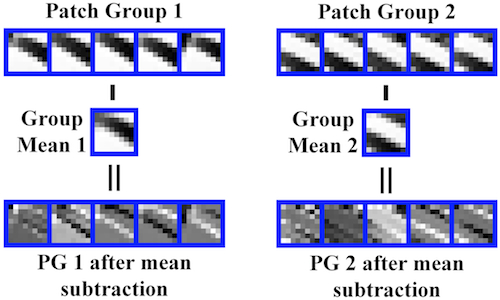
\includegraphics[width=.8\linewidth]{Figures/theory_pgpd/PG_subtract.jpg}
 	\caption{Different patch groups (PG) share similar PG variations.}
 	\label{fig:subtract_pgpd_1}
 \end{figure}

In order to find the best fit Gaussian component model for each PG, we check the posterior probability that $\overline{Y}$ belongs to the $k$th Gaussian component, denoted by $P(k|\overline{Y})$. Finally we simply choose the component which has the highest $P(k|\overline{Y})$ for this $\overline{Y}$. 

After selection for $\overline{Y}$, SVD is been applied to get the eigenvector matrix $\textbf{D}$ of $\Sigma$ which will be used as the dictionary.

\begin{equation}
	\Sigma = \textbf{D} \textbf{$\wedge$} \textbf{D}^T,
	\label{eq:pgpd_1}
\end{equation}

where \textbf{$\wedge$} represents the significance of these eigenvectors (Figure \ref{fig:eigen}). As we mention before, each patch in one PG has really similar variation after subtraction. So the $\textbf{D}$ actually represents the variation of the corresponding $\overline{Y}$. 

 \begin{figure}[H]
 	\centering
	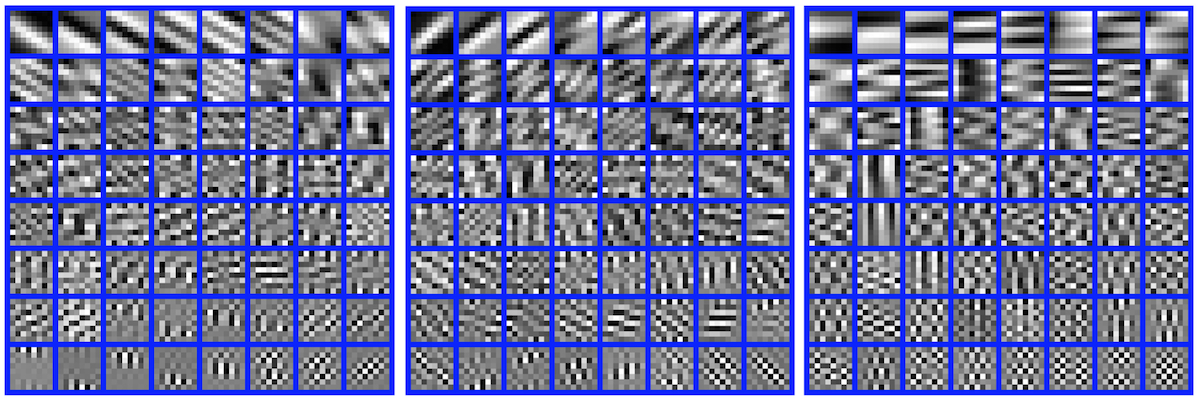
\includegraphics[width=.9\linewidth]{Figures/theory_pgpd/PG_eigenvector.jpg}
 	\caption{Eigenvectors $\textbf{D}$ of 3 different Gaussian components.}
 	\label{fig:eigen}
 \end{figure}
 
After \textbf{D} is acquired, we sparsely encode each patch $\overline{y}$ in the PG like below:

\begin{equation}
	\overline{y} = \textbf{D}* \alpha + \textbf{v},
	\label{eq:pgpd_2}
\end{equation}

$\alpha$ is the sparse coding coefficent. Since we assume noise $\textbf{v}$ as white Gaussian noise and $\alpha$ as i.i.d Laplacian distribution. And we already know $\overline{y}$ and $\textbf{D}$, so it is not that difficult to get $\alpha$.

Once acquiring $\alpha$, we simply get the denoised patch in the PG by $x = D\alpha + \mu$, where $\mu$ is the mean we subtract at the beginning of grouping patches. The big picture is below:

 \begin{figure}[H]
 	\centering
	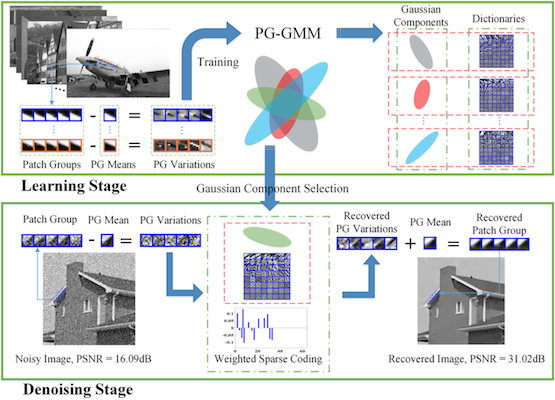
\includegraphics[width=\linewidth]{Figures/theory_pgpd/big_picture.jpg}
 	\caption{Whole process of PGPD method.}
 	\label{fig:subtract_pgpd}
 \end{figure}
%\section{Experimental Validation} \label{sc:experimental-validation}
In order to do a qualitative and quantitative analysis of the algorithms presented in Section \ref{sc:state-of-the-art}, a set of trials based on synthetic images was set up. The carried evaluation is twofold: (1) the algorithms were evaluated using synthetic images which were degenerated with a known type of noise and specific parameters for them; (2) we tested the different denoising techniques on retinopathy images. The complexity of denoising these images is that the kind of noise and its parameter are not known. Therefore, some noisy parameters have to be estimated.

\subsection{Synthetic images} \label{sc:experimental_sythetic}
When talking about synthetic images, one makes reference to those in which the level of noise is low.  The interest of using this kind of images for testing is that they have some characteristics related, for instance, to the content of high frequencies or low frequencies. Degenerated versions of these images can be used to evaluate the performance of denoising algorithms since the originals are known. To make the synthetic images, the three images shown in Fig. \ref{fig:setup_synthetic_originals} were noised in purpose. Cameraman image is characterised by having low frequencies, Lena image has intermediate frequencies and baboon image is composed by high frequencies. Therefore, using this images as a base of the synthetic images will give a proper analysis expanding the vast majority of the frequency range.

\begin{figure}[H]
  \centering
 \begin{tabular}{c c c c c}
     \begin{varwidth}{0.5\linewidth}
       \subfigure{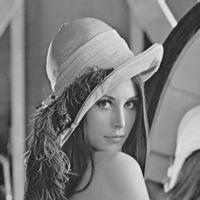
\includegraphics[width=16mm]{Figures/setup_synthetic_images/lena.jpg}}
     \end{varwidth}
     \begin{varwidth}{0.5\linewidth}
       \subfigure{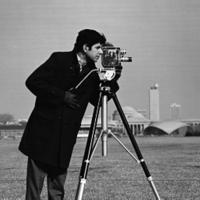
\includegraphics[width=16mm]{Figures/setup_synthetic_images/cameraman.jpg}}
     \end{varwidth}
     \begin{varwidth}{0.5\linewidth}
       \subfigure{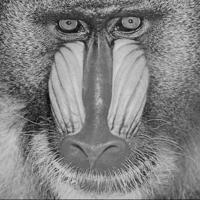
\includegraphics[width=16mm]{Figures/setup_synthetic_images/baboon.jpg}}
     \end{varwidth}
 \end{tabular}
  \caption{Original images. From left to right: Lena, cameraman and baboon.} 
  \label{fig:setup_synthetic_originals}
\end{figure}

Each one of these images was corrupted with 5 different types of noise: Gaussian, Rician, uniform, salt and pepper and speckle noise. While the first four types of noise are additive, the last one is multiplicative. Specifically, the characteristic parameters of each kind of noise are represented in Table \ref{tb:noising_parameters}.

\begin{table}[H]
    \centering
    \caption{Characteristics of the different types of noise.}
    \begin{tabular}{|c|c|}
    \hline
    \textbf{Type of noise} & \textbf{Characteristics} \\ \hline
    Gaussian & $\mu$=0 , $\sigma$=0.1 \\ \hline
    Rician & $\mu$=0.05 , $\sigma$=0.1 \\ \hline
    Uniform & $\mu$=0 , $\sigma$=0.1 \\ \hline
    Salt and Pepper & 5\% salt , 5\% pepper \\ \hline
    Speckle & $\mu$=0 , $\sigma$=0.04 \\ \hline
    \end{tabular}
    \label{tb:noising_parameters}
\end{table}

After applying the described noises in the original images seen in Fig. \ref{fig:setup_synthetic_originals}, the obtained noisy images are the ones shown in Fig. \ref{fig:setup_synthetic_noised}.

\begin{figure}[H]
  \centering
 \begin{tabular}{c c c c c}
     \begin{varwidth}{0.5\linewidth}
       \subfigure{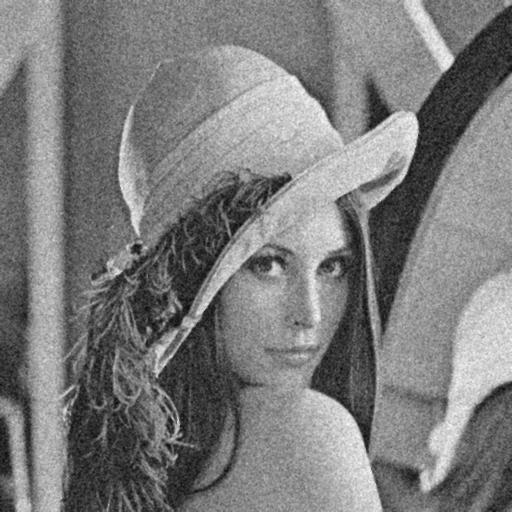
\includegraphics[width=16mm]{Figures/setup_synthetic_images/lena_nor.jpg}}\\
       \subfigure{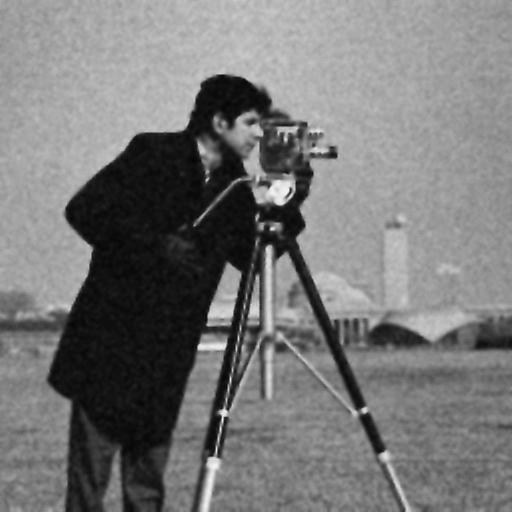
\includegraphics[width=16mm]{Figures/setup_synthetic_images/cameraman_nor.jpg}}\\
       \subfigure{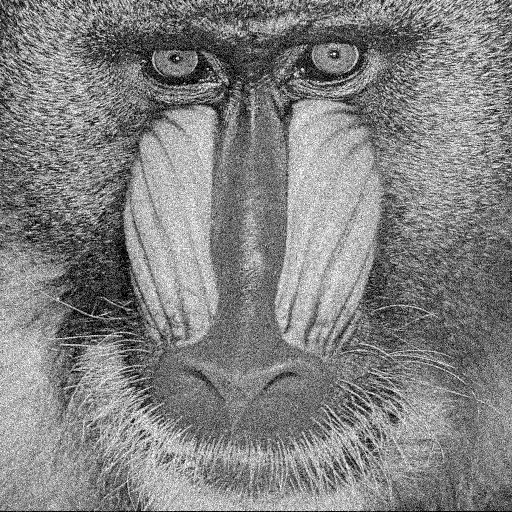
\includegraphics[width=16mm]{Figures/setup_synthetic_images/baboon_nor.jpg}}
     \end{varwidth}
     \begin{varwidth}{0.5\linewidth}
       \subfigure{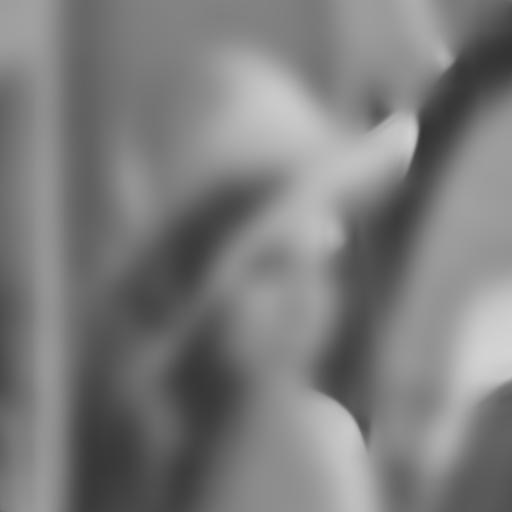
\includegraphics[width=16mm]{Figures/setup_synthetic_images/lena_ric.jpg}}\\
       \subfigure{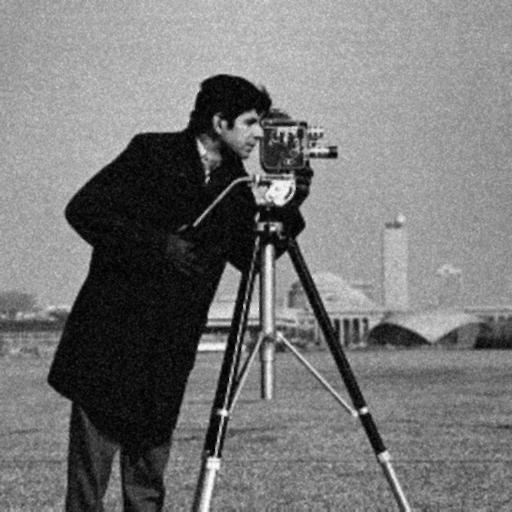
\includegraphics[width=16mm]{Figures/setup_synthetic_images/cameraman_ric.jpg}}\\
       \subfigure{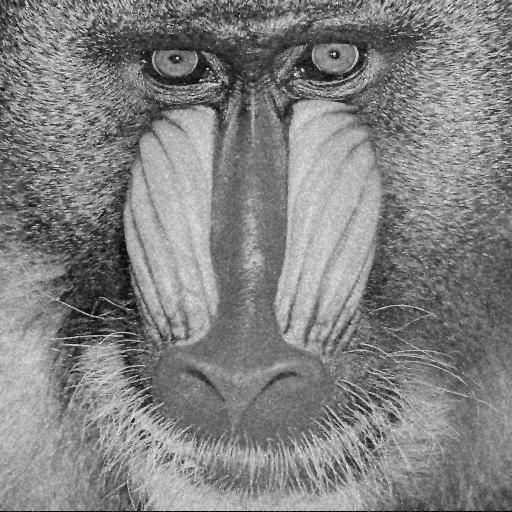
\includegraphics[width=16mm]{Figures/setup_synthetic_images/baboon_ric.jpg}}
     \end{varwidth}
     \begin{varwidth}{0.5\linewidth}
       \subfigure{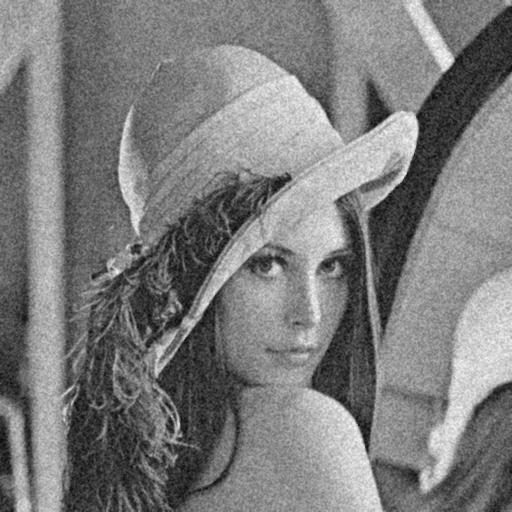
\includegraphics[width=16mm]{Figures/setup_synthetic_images/lena_uni.jpg}}\\
       \subfigure{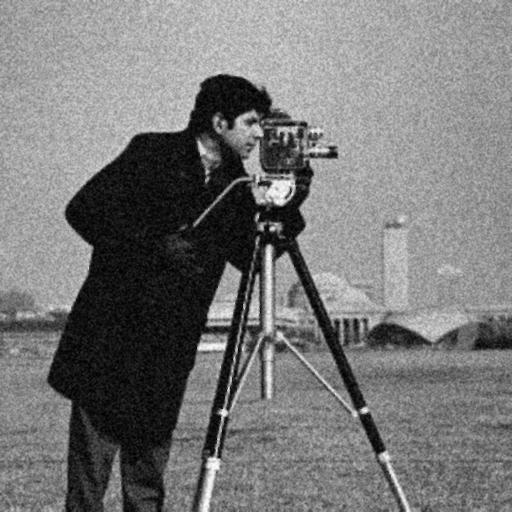
\includegraphics[width=16mm]{Figures/setup_synthetic_images/cameraman_uni.jpg}}\\
       \subfigure{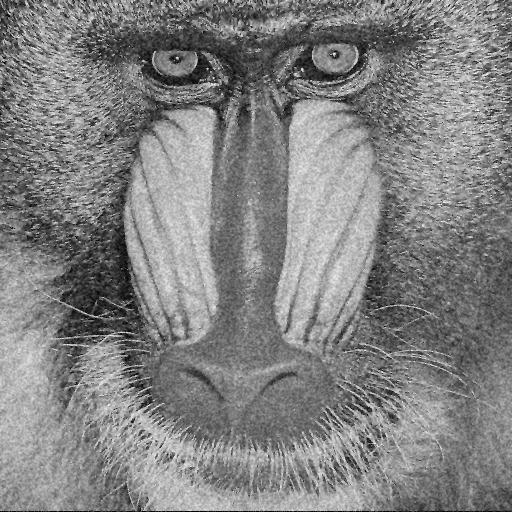
\includegraphics[width=16mm]{Figures/setup_synthetic_images/baboon_uni.jpg}}
     \end{varwidth}
     \begin{varwidth}{0.5\linewidth}
       \subfigure{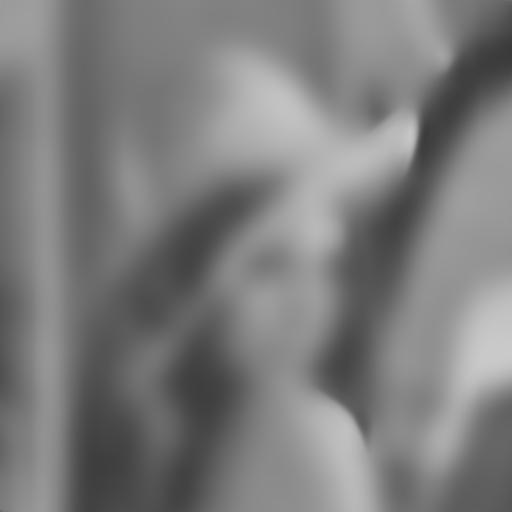
\includegraphics[width=16mm]{Figures/setup_synthetic_images/lena_sp.jpg}}\\
       \subfigure{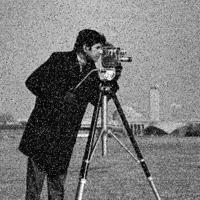
\includegraphics[width=16mm]{Figures/setup_synthetic_images/cameraman_sp.jpg}}\\
       \subfigure{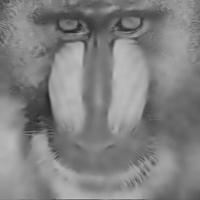
\includegraphics[width=16mm]{Figures/setup_synthetic_images/baboon_sp.jpg}}
     \end{varwidth}
     \begin{varwidth}{0.5\linewidth}
       \subfigure{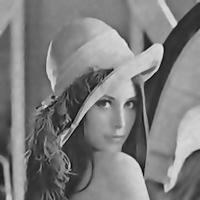
\includegraphics[width=16mm]{Figures/setup_synthetic_images/lena_spec.jpg}}\\
       \subfigure{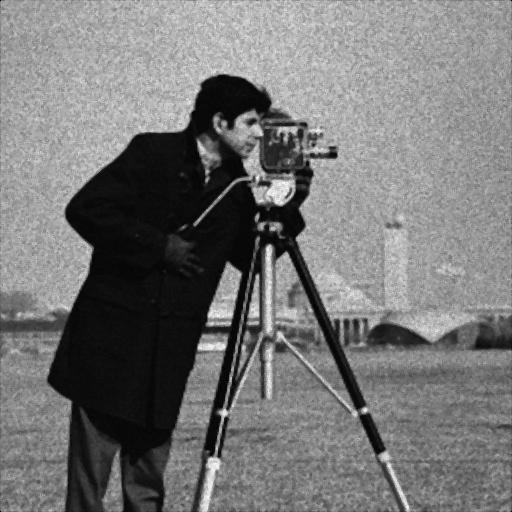
\includegraphics[width=16mm]{Figures/setup_synthetic_images/cameraman_spec.jpg}}\\
       \subfigure{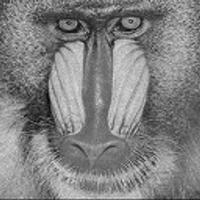
\includegraphics[width=16mm]{Figures/setup_synthetic_images/baboon_spec.jpg}}
     \end{varwidth}
 \end{tabular}
  \caption{Noised images. From left to right: additive Gaussian, additive Rician, additive uniform, additive salt and pepper and multiplicative speckle noise, respectively.} 
  \label{fig:setup_synthetic_noised}
\end{figure}

For visualization purposes, all the images shown in Section \ref{sc:results} will be shown in a colormap format. As can be seen in Fig. \ref{fig:setup_synthetic_noised_color}, the noise added to the images in Fig. \ref{fig:setup_synthetic_noised} can be better with this color visualization. 

\begin{figure}[H]
  \centering
 \begin{tabular}{c c c c c}
     \begin{varwidth}{0.5\linewidth}
       \subfigure{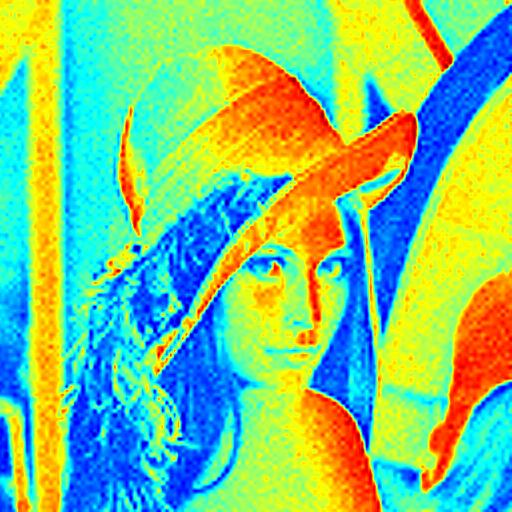
\includegraphics[width=16mm]{Figures/setup_synthetic_images/color_lena_nor.jpg}}\\
       \subfigure{\includegraphics[width=16mm]{Figures/setup_synthetic_images/color_cameraman_nor.jpg}}\\
       \subfigure{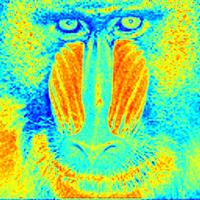
\includegraphics[width=16mm]{Figures/setup_synthetic_images/color_baboon_nor.jpg}}
     \end{varwidth}
     \begin{varwidth}{0.5\linewidth}
       \subfigure{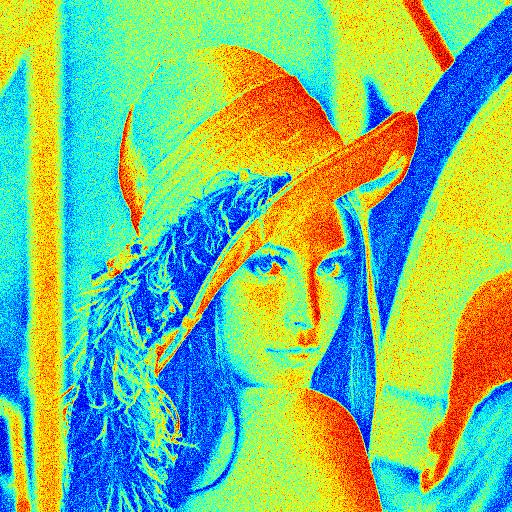
\includegraphics[width=16mm]{Figures/setup_synthetic_images/color_lena_ric.jpg}}\\
       \subfigure{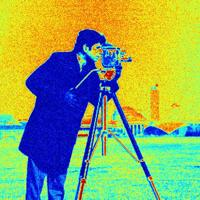
\includegraphics[width=16mm]{Figures/setup_synthetic_images/color_cameraman_ric.jpg}}\\
       \subfigure{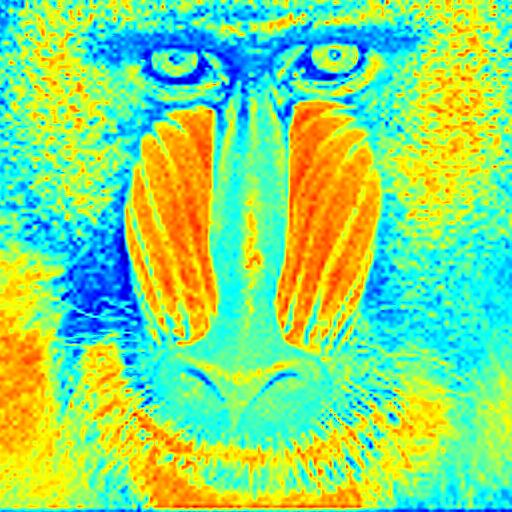
\includegraphics[width=16mm]{Figures/setup_synthetic_images/color_baboon_ric.jpg}}
     \end{varwidth}
     \begin{varwidth}{0.5\linewidth}
       \subfigure{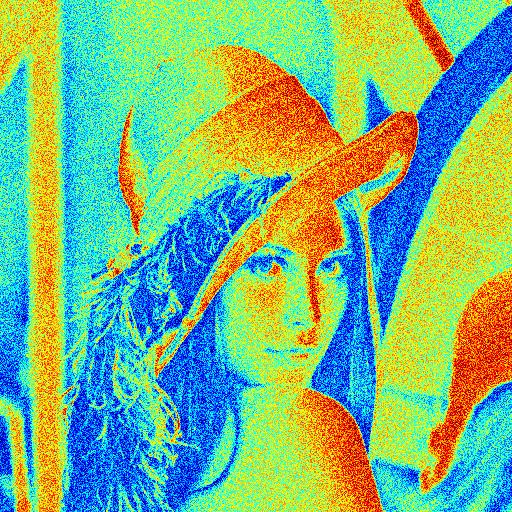
\includegraphics[width=16mm]{Figures/setup_synthetic_images/color_lena_uni.jpg}}\\
       \subfigure{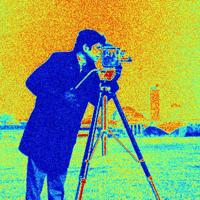
\includegraphics[width=16mm]{Figures/setup_synthetic_images/color_cameraman_uni.jpg}}\\
       \subfigure{\includegraphics[width=16mm]{Figures/setup_synthetic_images/color_baboon_uni.jpg}}
     \end{varwidth}
     \begin{varwidth}{0.5\linewidth}
       \subfigure{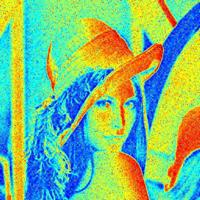
\includegraphics[width=16mm]{Figures/setup_synthetic_images/color_lena_sp.jpg}}\\
       \subfigure{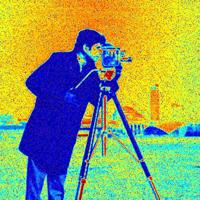
\includegraphics[width=16mm]{Figures/setup_synthetic_images/color_cameraman_sp.jpg}}\\
       \subfigure{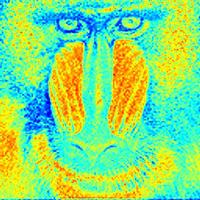
\includegraphics[width=16mm]{Figures/setup_synthetic_images/color_baboon_sp.jpg}}
     \end{varwidth}
     \begin{varwidth}{0.5\linewidth}
       \subfigure{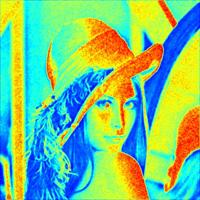
\includegraphics[width=16mm]{Figures/setup_synthetic_images/color_lena_spec.jpg}}\\
       \subfigure{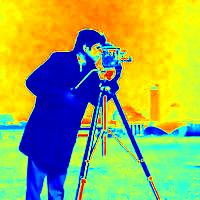
\includegraphics[width=16mm]{Figures/setup_synthetic_images/color_cameraman_spec.jpg}}\\
       \subfigure{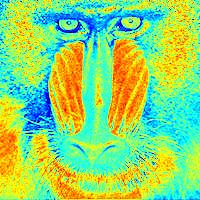
\includegraphics[width=16mm]{Figures/setup_synthetic_images/color_baboon_spec.jpg}}
     \end{varwidth}
 \end{tabular}
  \caption{Noised images represented in a colormap format. From left to right: additive Gaussian, additive Rician, additive uniform, additive salt and pepper and multiplicative speckle noise, respectively.} 
  \label{fig:setup_synthetic_noised_color}
\end{figure}

\subsection{Retinopathy images}
In the previous section, we presented an evaluation based on noising synthetic images in which the noise characteristics were known in advance. However, these parameters are usually not given in real-life scenarios. To evaluate the algorithm under this kind of conditions, we consider Spatial-Domain Optical coherence tomography (SD-OCT) images. The evaluation using these images consists of the following steps. First, a volume of OCT is taken and processed using the different considered algorithms. For this task, we consider the dataset provided by the University of Girona \cite{udg}. Second, the noise is estimated and the determined value is used as input for the K-SVD algorithm. 

\begin{figure}[H]
  \centering
      \subfigure{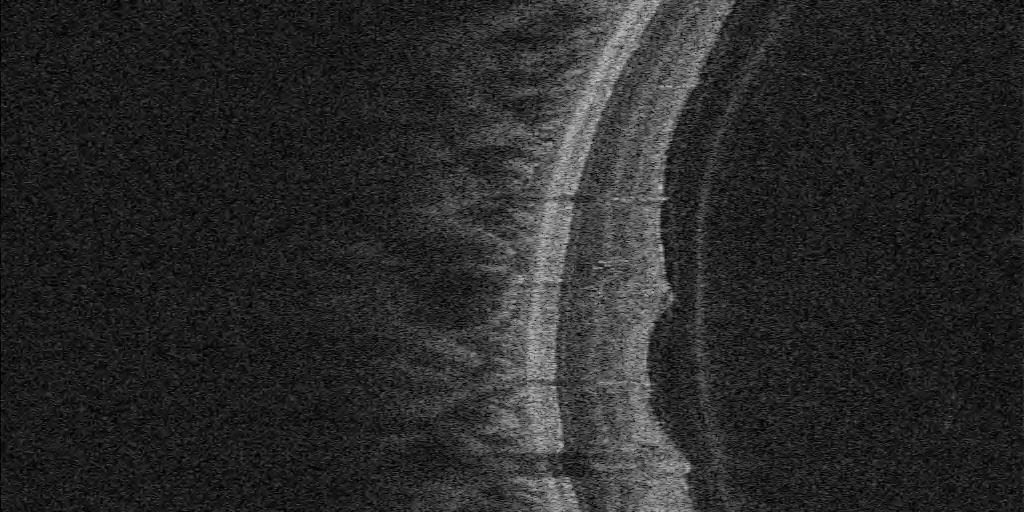
\includegraphics[width=80mm]{Figures/setup_retinopathy/original_P741009OS.jpg}}
  \caption{Retinopathy image.} 
  \label{fig:setup_retinopathy_image_setup}
\end{figure}

The goal of denoising retinopathy images is to obtain a better segmentation of the different retinopathy layers. For this, the resulting denoised images are segmented using the tool called OCT Explorer developed by the University of Iowa \cite{iowa}. Finally, the outcome of the segmentation is compared against the segmentation of the noisy retinopathy volume, which can be seen in Fig. \ref{fig:setup_retinopathy_segmentation_setup}.

\begin{figure}[H]
  \centering
      \subfigure{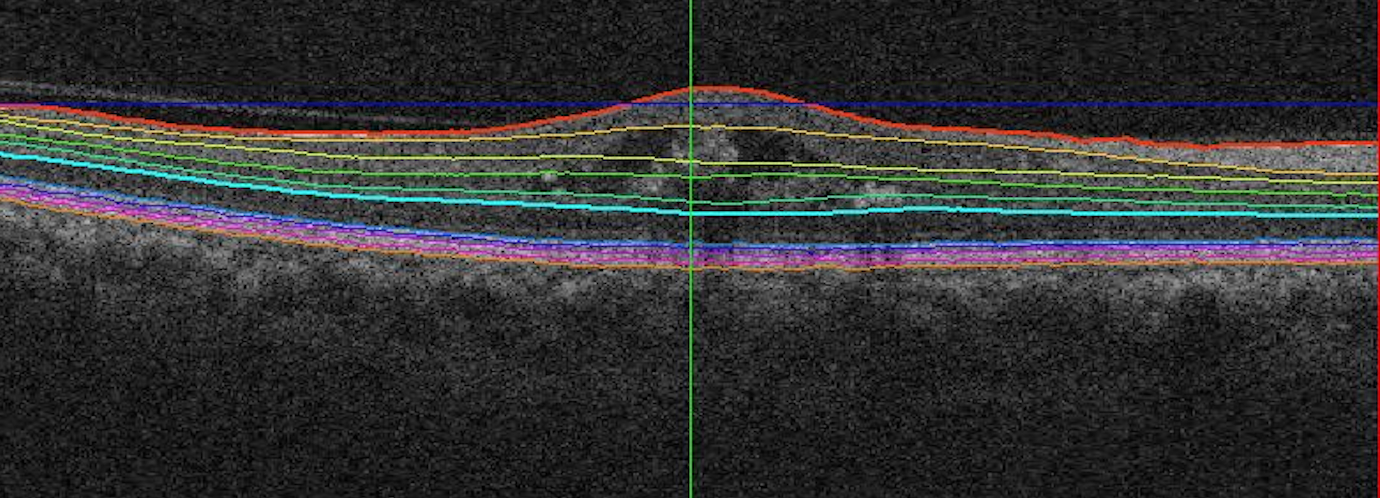
\includegraphics[width=80mm]{Figures/setup_retinopathy/original_segmentation.jpg}}
  \caption{Segmentation of a noisy retinopathy volume.} 
  \label{fig:setup_retinopathy_segmentation_setup}
\end{figure}

The output segmentation of the noisy volume shows up all the 11 existing layers of the retina. Since there is not any ground-truth to check the accuracy of the resulting segmentations, only the number of obtained layers and a visual analysis can be given in the following analysis.  
\section{Results} \label{sc:results}
Ȉric: setting this section offline (due to Overleaf limitation). Available in GitHub

\subsection{Synthetic images}

\subsubsection{KSVD}

\begin{figure}[H]
  \centering
  \begin{tabular}{c c c c c}
      \begin{varwidth}{0.5\linewidth}
        \subfigure{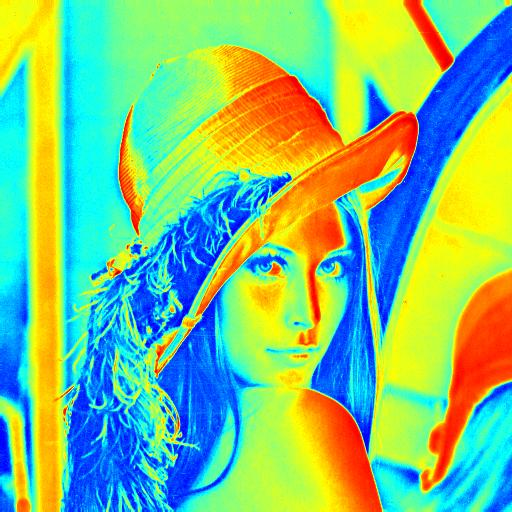
\includegraphics[width=16mm]{Experiments_synthetic_images/color_lena.jpg}}\\
        \subfigure{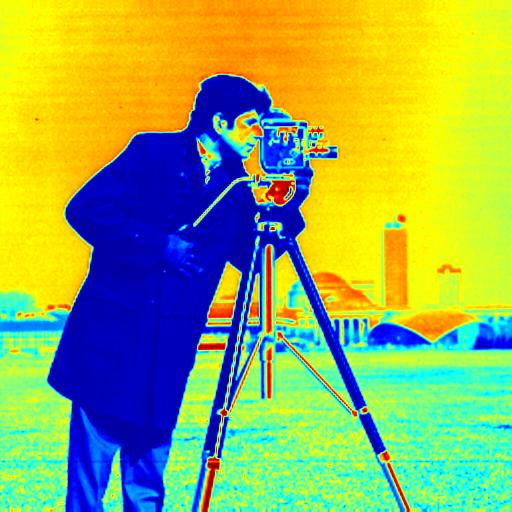
\includegraphics[width=16mm]{Experiments_synthetic_images/color_cameraman.jpg}}\\
        \subfigure{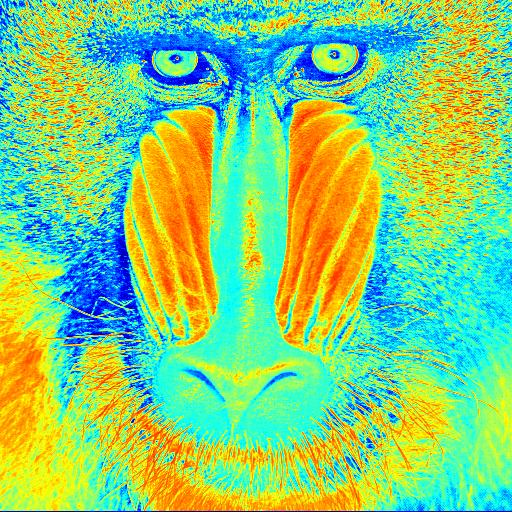
\includegraphics[width=16mm]{Experiments_synthetic_images/color_baboon.jpg}}
      \end{varwidth}
      \begin{varwidth}{0.5\linewidth}
        \subfigure{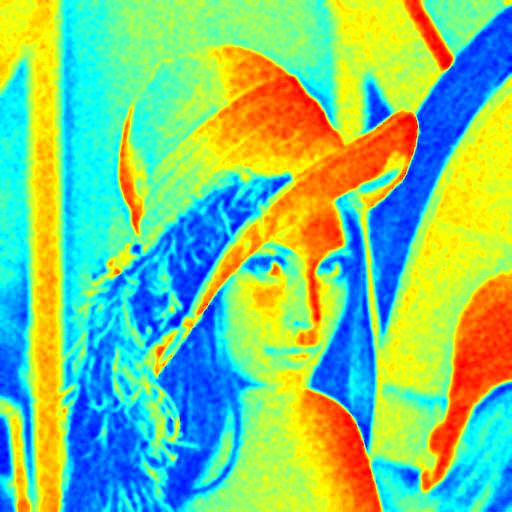
\includegraphics[width=16mm]{Results_KSVD/color_lena_nor.jpg}}\\
        \subfigure{\includegraphics[width=16mm]{Results_KSVD/color_cameraman_nor.jpg}}\\
        \subfigure{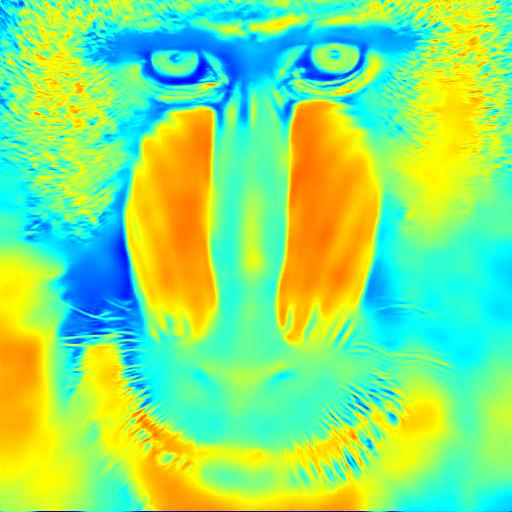
\includegraphics[width=16mm]{Results_KSVD/color_baboon_nor.jpg}}
      \end{varwidth}
      \begin{varwidth}{0.5\linewidth}
        \subfigure{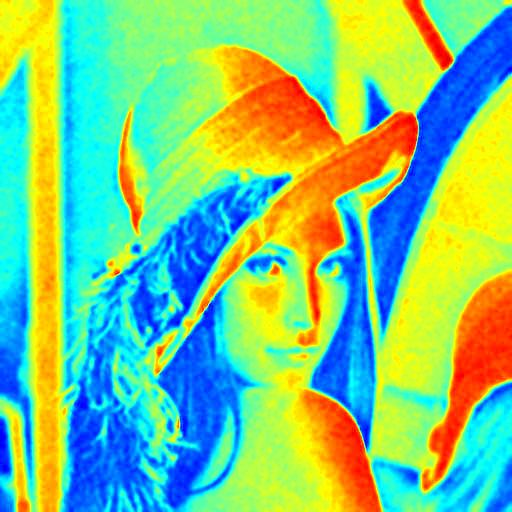
\includegraphics[width=16mm]{Results_KSVD/color_lena_ric.jpg}}\\
        \subfigure{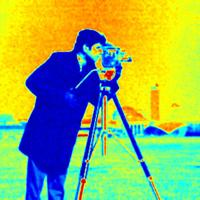
\includegraphics[width=16mm]{Results_KSVD/color_cameraman_ric.jpg}}\\
        \subfigure{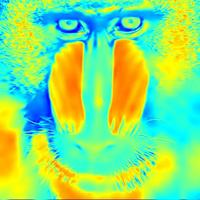
\includegraphics[width=16mm]{Results_KSVD/color_baboon_ric.jpg}}
      \end{varwidth}
      \begin{varwidth}{0.5\linewidth}
        \subfigure{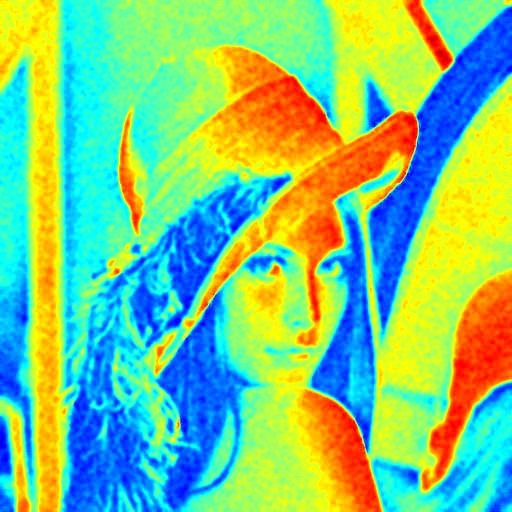
\includegraphics[width=16mm]{Results_KSVD/color_lena_uni.jpg}}\\
        \subfigure{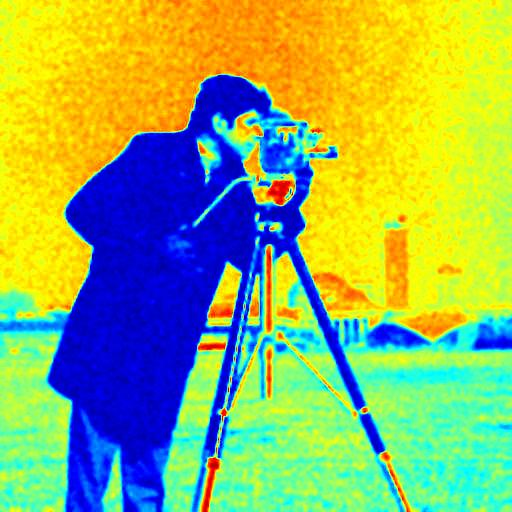
\includegraphics[width=16mm]{Results_KSVD/color_cameraman_uni.jpg}}\\
        \subfigure{\includegraphics[width=16mm]{Results_KSVD/color_baboon_uni.jpg}}
      \end{varwidth}
      \begin{varwidth}{0.5\linewidth}
        \subfigure{\includegraphics[width=16mm]{Results_KSVD/color_lena_sp.jpg}}\\
        \subfigure{\includegraphics[width=16mm]{Results_KSVD/color_cameraman_sp.jpg}}\\
        \subfigure{\includegraphics[width=16mm]{Results_KSVD/color_baboon_sp.jpg}}
      \end{varwidth}
  	\end{tabular}
  \caption{} 
  \label{fig:results_ksvd_c}
\end{figure}

\subsubsection{Mean filter}

\begin{figure}[H]
  \centering
  \begin{tabular}{c c c c c}
      \begin{varwidth}{0.5\linewidth}
        \subfigure{\includegraphics[width=16mm]{Experiments_synthetic_images/color_lena.jpg}}\\
        \subfigure{\includegraphics[width=16mm]{Experiments_synthetic_images/color_cameraman.jpg}}\\
        \subfigure{\includegraphics[width=16mm]{Experiments_synthetic_images/color_baboon.jpg}}
      \end{varwidth}
      \begin{varwidth}{0.5\linewidth}
        \subfigure{\includegraphics[width=16mm]{Results_mean/color_lena_nor_f.jpg}}\\
        \subfigure{\includegraphics[width=16mm]{Results_mean/color_cameraman_nor_f.jpg}}\\
        \subfigure{\includegraphics[width=16mm]{Results_mean/color_baboon_nor_f.jpg}}
      \end{varwidth}
      \begin{varwidth}{0.5\linewidth}
        \subfigure{\includegraphics[width=16mm]{Results_mean/color_lena_ric_f.jpg}}\\
        \subfigure{\includegraphics[width=16mm]{Results_mean/color_cameraman_ric_f.jpg}}\\
        \subfigure{\includegraphics[width=16mm]{Results_mean/color_baboon_ric_f.jpg}}
      \end{varwidth}
      \begin{varwidth}{0.5\linewidth}
        \subfigure{\includegraphics[width=16mm]{Results_mean/color_lena_uni_f.jpg}}\\
        \subfigure{\includegraphics[width=16mm]{Results_mean/color_cameraman_uni_f.jpg}}\\
        \subfigure{\includegraphics[width=16mm]{Results_mean/color_baboon_uni_f.jpg}}
      \end{varwidth}
      \begin{varwidth}{0.5\linewidth}
        \subfigure{\includegraphics[width=16mm]{Results_mean/color_lena_sp_f.jpg}}\\
        \subfigure{\includegraphics[width=16mm]{Results_mean/color_cameraman_sp_f.jpg}}\\
        \subfigure{\includegraphics[width=16mm]{Results_mean/color_baboon_sp_f.jpg}}
      \end{varwidth}
  	\end{tabular}
  \caption{} 
  \label{fig:results_mean_c}
\end{figure}

compare with KSVD results

\subsubsection{Median filter}

\begin{figure}[H]
  \centering
  \begin{tabular}{c c c c c}
      \begin{varwidth}{0.5\linewidth}
        \subfigure{\includegraphics[width=16mm]{Experiments_synthetic_images/color_lena.jpg}}\\
        \subfigure{\includegraphics[width=16mm]{Experiments_synthetic_images/color_cameraman.jpg}}\\
        \subfigure{\includegraphics[width=16mm]{Experiments_synthetic_images/color_baboon.jpg}}
      \end{varwidth}
      \begin{varwidth}{0.5\linewidth}
        \subfigure{\includegraphics[width=16mm]{Results_median/color_lena_nor_f.jpg}}\\
        \subfigure{\includegraphics[width=16mm]{Results_median/color_cameraman_nor_f.jpg}}\\
        \subfigure{\includegraphics[width=16mm]{Results_median/color_baboon_nor_f.jpg}}
      \end{varwidth}
      \begin{varwidth}{0.5\linewidth}
        \subfigure{\includegraphics[width=16mm]{Results_median/color_lena_ric_f.jpg}}\\
        \subfigure{\includegraphics[width=16mm]{Results_median/color_cameraman_ric_f.jpg}}\\
        \subfigure{\includegraphics[width=16mm]{Results_median/color_baboon_ric_f.jpg}}
      \end{varwidth}
      \begin{varwidth}{0.5\linewidth}
        \subfigure{\includegraphics[width=16mm]{Results_median/color_lena_uni_f.jpg}}\\
        \subfigure{\includegraphics[width=16mm]{Results_median/color_cameraman_uni_f.jpg}}\\
        \subfigure{\includegraphics[width=16mm]{Results_median/color_baboon_uni_f.jpg}}
      \end{varwidth}
      \begin{varwidth}{0.5\linewidth}
        \subfigure{\includegraphics[width=16mm]{Results_median/color_lena_sp_f.jpg}}\\
        \subfigure{\includegraphics[width=16mm]{Results_median/color_cameraman_sp_f.jpg}}\\
        \subfigure{\includegraphics[width=16mm]{Results_median/color_baboon_sp_f.jpg}}
      \end{varwidth}
  	\end{tabular}
  \caption{} 
  \label{fig:results_median_c}
\end{figure}

compare with KSVD results

\subsubsection{Lee filter}
add images denoised with lee
compare with KSVD results

\subsubsection{Hard and soft thresholding in wavelet domain}

\begin{figure}[H]
  \centering
  \begin{tabular}{c c c c c}
      \begin{varwidth}{0.5\linewidth}
        \subfigure{\includegraphics[width=16mm]{Experiments_synthetic_images/color_lena.jpg}}\\
        \subfigure{\includegraphics[width=16mm]{Experiments_synthetic_images/color_cameraman.jpg}}\\
        \subfigure{\includegraphics[width=16mm]{Experiments_synthetic_images/color_baboon.jpg}}
      \end{varwidth}
      \begin{varwidth}{0.5\linewidth}
        \subfigure{\includegraphics[width=16mm]{Results_wavelet/color_lena_nor.jpg}}\\
        \subfigure{\includegraphics[width=16mm]{Results_wavelet/color_cameraman_nor.jpg}}\\
        \subfigure{\includegraphics[width=16mm]{Results_wavelet/color_baboon_nor.jpg}}
      \end{varwidth}
      \begin{varwidth}{0.5\linewidth}
        \subfigure{\includegraphics[width=16mm]{Results_wavelet/color_lena_ric.jpg}}\\
        \subfigure{\includegraphics[width=16mm]{Results_wavelet/color_cameraman_ric.jpg}}\\
        \subfigure{\includegraphics[width=16mm]{Results_wavelet/color_baboon_ric.jpg}}
      \end{varwidth}
      \begin{varwidth}{0.5\linewidth}
        \subfigure{\includegraphics[width=16mm]{Results_wavelet/color_lena_uni.jpg}}\\
        \subfigure{\includegraphics[width=16mm]{Results_wavelet/color_cameraman_uni.jpg}}\\
        \subfigure{\includegraphics[width=16mm]{Results_wavelet/color_baboon_uni.jpg}}
      \end{varwidth}
      \begin{varwidth}{0.5\linewidth}
        \subfigure{\includegraphics[width=16mm]{Results_wavelet/color_lena_sp.jpg}}\\
        \subfigure{\includegraphics[width=16mm]{Results_wavelet/color_cameraman_sp.jpg}}\\
        \subfigure{\includegraphics[width=16mm]{Results_wavelet/color_baboon_sp.jpg}}
      \end{varwidth}
  	\end{tabular}
  \caption{} 
  \label{fig:results_wavelet_c}
\end{figure}

compare with KSVD results

\subsection{Retinopathy images} 



%\section{Final remarks} \label{sc:final-remarks}
The K-SVD algorithm was compared against different well-known techniques for denoising images such as mean, median, lee and wavelet-based filter. The algorithm was analysed in terms of the influence of its parameters on the results and, also, on its capability to remove noise.

The evaluation showed that the K-SVD algorithm was able to denoise synthetic and SD-OCT images achieving better results in some cases compared to the other algorithms.  Although noise was reduced, the segmentation carried out on an OCT volume evidenced that no significant improvement was observed between noisy and denoised images.

The K-SVD algorithm is recommended for removing noise on SD-OCT images since, in terms of PSNR, the results were the best. However, further evaluation on the segmentation section should be done in order to determine the best parameters for this task.

\section{Appendices}
In this appendix are included all the original black and white denoised images and its PSNR values. 

\begin{figure}[H]
  \centering
  \begin{tabular}{c c c c c}
      \begin{varwidth}{0.5\linewidth}
        \subfigure{\includegraphics[width=16mm]{Figures/results_mean/lena_nor_f.jpg}}\\
        \subfigure{\includegraphics[width=16mm]{Figures/results_mean/cameraman_nor_f.jpg}}\\
        \subfigure{\includegraphics[width=16mm]{Figures/results_mean/baboon_nor_f.jpg}}
      \end{varwidth}
      \begin{varwidth}{0.5\linewidth}
        \subfigure{\includegraphics[width=16mm]{Figures/results_mean/lena_ric_f.jpg}}\\
        \subfigure{\includegraphics[width=16mm]{Figures/results_mean/cameraman_ric_f.jpg}}\\
        \subfigure{\includegraphics[width=16mm]{Figures/results_mean/baboon_ric_f.jpg}}
      \end{varwidth}
      \begin{varwidth}{0.5\linewidth}
        \subfigure{\includegraphics[width=16mm]{Figures/results_mean/lena_uni_f.jpg}}\\
        \subfigure{\includegraphics[width=16mm]{Figures/results_mean/cameraman_uni_f.jpg}}\\
        \subfigure{\includegraphics[width=16mm]{Figures/results_mean/baboon_uni_f.jpg}}
      \end{varwidth}
      \begin{varwidth}{0.5\linewidth}
        \subfigure{\includegraphics[width=16mm]{Figures/results_mean/lena_sp_f.jpg}}\\
        \subfigure{\includegraphics[width=16mm]{Figures/results_mean/cameraman_sp_f.jpg}}\\
        \subfigure{\includegraphics[width=16mm]{Figures/results_mean/baboon_sp_f.jpg}}
      \end{varwidth}
      \begin{varwidth}{0.5\linewidth}
        \subfigure{\includegraphics[width=16mm]{Figures/results_mean/lena_spec.jpg}}\\
        \subfigure{\includegraphics[width=16mm]{Figures/results_mean/cameraman_spec.jpg}}\\
        \subfigure{\includegraphics[width=16mm]{Figures/results_mean/baboon_spec.jpg}}
      \end{varwidth}
  	\end{tabular}
  \caption{Denoised images with the mean filter. From left to right: removing Gaussian, Rician, uniform, salt and pepper and speckle noise, respectively.} 
  \label{fig:results_synthetic_mean}
\end{figure}

\begin{figure}[H]
  \centering
  \begin{tabular}{c c c c c}
      \begin{varwidth}{0.5\linewidth}
        \subfigure{\includegraphics[width=16mm]{Figures/results_median/lena_nor_f.jpg}}\\
        \subfigure{\includegraphics[width=16mm]{Figures/results_median/cameraman_nor_f.jpg}}\\
        \subfigure{\includegraphics[width=16mm]{Figures/results_median/baboon_nor_f.jpg}}
      \end{varwidth}
      \begin{varwidth}{0.5\linewidth}
        \subfigure{\includegraphics[width=16mm]{Figures/results_median/lena_ric_f.jpg}}\\
        \subfigure{\includegraphics[width=16mm]{Figures/results_median/cameraman_ric_f.jpg}}\\
        \subfigure{\includegraphics[width=16mm]{Figures/results_median/baboon_ric_f.jpg}}
      \end{varwidth}
      \begin{varwidth}{0.5\linewidth}
        \subfigure{\includegraphics[width=16mm]{Figures/results_median/lena_uni_f.jpg}}\\
        \subfigure{\includegraphics[width=16mm]{Figures/results_median/cameraman_uni_f.jpg}}\\
        \subfigure{\includegraphics[width=16mm]{Figures/results_median/baboon_uni_f.jpg}}
      \end{varwidth}
      \begin{varwidth}{0.5\linewidth}
        \subfigure{\includegraphics[width=16mm]{Figures/results_median/lena_sp_f.jpg}}\\
        \subfigure{\includegraphics[width=16mm]{Figures/results_median/cameraman_sp_f.jpg}}\\
        \subfigure{\includegraphics[width=16mm]{Figures/results_median/baboon_sp_f.jpg}}
      \end{varwidth}
      \begin{varwidth}{0.5\linewidth}
        \subfigure{\includegraphics[width=16mm]{Figures/results_median/lena_spec.jpg}}\\
        \subfigure{\includegraphics[width=16mm]{Figures/results_median/cameraman_spec.jpg}}\\
        \subfigure{\includegraphics[width=16mm]{Figures/results_median/baboon_spec.jpg}}
      \end{varwidth}
  	\end{tabular}
  \caption{Denoised images with the median filter. From left to right: removing Gaussian, Rician, uniform, salt and pepper and speckle noise, respectively.} 
  \label{fig:results_synthetic_median}
\end{figure}

\begin{figure}[H]
  \centering
  \begin{tabular}{c c c c c}
      \begin{varwidth}{0.5\linewidth}
        \subfigure{\includegraphics[width=16mm]{Figures/results_Lee/lena_nor-denoised.jpg}}\\
        \subfigure{\includegraphics[width=16mm]{Figures/results_Lee/cameraman_nor-denoised.jpg}}\\
        \subfigure{\includegraphics[width=16mm]{Figures/results_Lee/baboon_nor-denoised.jpg}}
      \end{varwidth}
      \begin{varwidth}{0.5\linewidth}
        \subfigure{\includegraphics[width=16mm]{Figures/results_Lee/lena_ric-denoised.jpg}}\\
        \subfigure{\includegraphics[width=16mm]{Figures/results_Lee/cameraman_ric-denoised.jpg}}\\
        \subfigure{\includegraphics[width=16mm]{Figures/results_Lee/baboon_ric-denoised.jpg}}
      \end{varwidth}
      \begin{varwidth}{0.5\linewidth}
        \subfigure{\includegraphics[width=16mm]{Figures/results_Lee/lena_uni-denoised.jpg}}\\
        \subfigure{\includegraphics[width=16mm]{Figures/results_Lee/cameraman_uni-denoised.jpg}}\\
        \subfigure{\includegraphics[width=16mm]{Figures/results_Lee/baboon_uni-denoised.jpg}}
      \end{varwidth}
      \begin{varwidth}{0.5\linewidth}
        \subfigure{\includegraphics[width=16mm]{Figures/results_Lee/lena_sp-denoised.jpg}}\\
        \subfigure{\includegraphics[width=16mm]{Figures/results_Lee/cameraman_sp-denoised.jpg}}\\
        \subfigure{\includegraphics[width=16mm]{Figures/results_Lee/baboon_sp-denoised.jpg}}
      \end{varwidth}
      \begin{varwidth}{0.5\linewidth}
        \subfigure{\includegraphics[width=16mm]{Figures/results_Lee/lena_spec.jpg}}\\
        \subfigure{\includegraphics[width=16mm]{Figures/results_Lee/cameraman_spec.jpg}}\\
        \subfigure{\includegraphics[width=16mm]{Figures/results_Lee/baboon_spec.jpg}}
      \end{varwidth}
  	\end{tabular}
  \caption{Denoised images with the LS filter. From left to right: removing Gaussian, Rician, uniform, salt and pepper and speckle noise, respectively.} 
  \label{fig:results_synthetic_ls}
\end{figure}

\begin{figure}[H]
  \centering
  \begin{tabular}{c c c c c}
      \begin{varwidth}{0.5\linewidth}
        \subfigure{\includegraphics[width=16mm]{Figures/results_wavelet/lena_nor.jpg}}\\
        \subfigure{\includegraphics[width=16mm]{Figures/results_wavelet/cameraman_nor.jpg}}\\
        \subfigure{\includegraphics[width=16mm]{Figures/results_wavelet/baboon_nor.jpg}}
      \end{varwidth}
      \begin{varwidth}{0.5\linewidth}
        \subfigure{\includegraphics[width=16mm]{Figures/results_wavelet/lena_ric.jpg}}\\
        \subfigure{\includegraphics[width=16mm]{Figures/results_wavelet/cameraman_ric.jpg}}\\
        \subfigure{\includegraphics[width=16mm]{Figures/results_wavelet/baboon_ric.jpg}}
      \end{varwidth}
      \begin{varwidth}{0.5\linewidth}
        \subfigure{\includegraphics[width=16mm]{Figures/results_wavelet/lena_uni.jpg}}\\
        \subfigure{\includegraphics[width=16mm]{Figures/results_wavelet/cameraman_uni.jpg}}\\
        \subfigure{\includegraphics[width=16mm]{Figures/results_wavelet/baboon_uni.jpg}}
      \end{varwidth}
      \begin{varwidth}{0.5\linewidth}
        \subfigure{\includegraphics[width=16mm]{Figures/results_wavelet/lena_sp.jpg}}\\
        \subfigure{\includegraphics[width=16mm]{Figures/results_wavelet/cameraman_sp.jpg}}\\
        \subfigure{\includegraphics[width=16mm]{Figures/results_wavelet/baboon_sp.jpg}}
      \end{varwidth}
      \begin{varwidth}{0.5\linewidth}
        \subfigure{\includegraphics[width=16mm]{Figures/results_wavelet/lena_spec.jpg}}\\
        \subfigure{\includegraphics[width=16mm]{Figures/results_wavelet/cameraman_spec.jpg}}\\
        \subfigure{\includegraphics[width=16mm]{Figures/results_wavelet/baboon_spec.jpg}}
      \end{varwidth}
  	\end{tabular}
  \caption{Denoised images with the wavelet filter. From left to right: removing Gaussian, Rician, uniform, salt and pepper and speckle noise, respectively.} 
  \label{fig:results_synthetic_wavelet}
\end{figure}

\begin{figure}[H]
  \centering
 \begin{tabular}{c c c c c}
     \begin{varwidth}{0.5\linewidth}
       \subfigure{\includegraphics[width=16mm]{Figures/results_KSVD/lena_nor.jpg}}\\
       \subfigure{\includegraphics[width=16mm]{Figures/results_KSVD/cameraman_nor.jpg}}\\
       \subfigure{\includegraphics[width=16mm]{Figures/results_KSVD/baboon_nor.jpg}}
     \end{varwidth}
     \begin{varwidth}{0.5\linewidth}
       \subfigure{\includegraphics[width=16mm]{Figures/results_KSVD/lena_ric.jpg}}\\
       \subfigure{\includegraphics[width=16mm]{Figures/results_KSVD/cameraman_ric.jpg}}\\
       \subfigure{\includegraphics[width=16mm]{Figures/results_KSVD/baboon_ric.jpg}}
     \end{varwidth}
     \begin{varwidth}{0.5\linewidth}
       \subfigure{\includegraphics[width=16mm]{Figures/results_KSVD/lena_uni.jpg}}\\
       \subfigure{\includegraphics[width=16mm]{Figures/results_KSVD/cameraman_uni.jpg}}\\
       \subfigure{\includegraphics[width=16mm]{Figures/results_KSVD/baboon_uni.jpg}}
     \end{varwidth}
     \begin{varwidth}{0.5\linewidth}
       \subfigure{\includegraphics[width=16mm]{Figures/results_KSVD/lena_sp.jpg}}\\
       \subfigure{\includegraphics[width=16mm]{Figures/results_KSVD/cameraman_sp.jpg}}\\
       \subfigure{\includegraphics[width=16mm]{Figures/results_KSVD/baboon_sp.jpg}}
     \end{varwidth}
     \begin{varwidth}{0.5\linewidth}
       \subfigure{\includegraphics[width=16mm]{Figures/results_KSVD/lena_spec.jpg}}\\
       \subfigure{\includegraphics[width=16mm]{Figures/results_KSVD/cameraman_spec.jpg}}\\
       \subfigure{\includegraphics[width=16mm]{Figures/results_KSVD/baboon_spec.jpg}}
     \end{varwidth}
 	\end{tabular}
  \caption{Denoised images with the K-SVD filter. From left to right: removing Gaussian, Rician, uniform, salt and pepper and speckle noise, respectively.} 
  \label{fig:results_synthetic_K-SVD}
\end{figure}

In order to easily compare the performance of the different methods, the PSNR results have been grouped according to the different kind of noise that have been analyzed.

\begin{table}[H]
	\centering
	\caption{PSNR for denoising algorithms considering Gaussian noise}
	\begin{tabular}{|c|c|c|c|}
	\hline
	\textbf{Technique} & \textbf{Lena} & \textbf{Cameraman} & \textbf{Baboon} \\ \hline
	Mean & $28.54$ & $28.64$ & $21.77$ \\ \hline
	Median & $27.59$ & $27.88$ & $21.60$ \\ \hline
	LS & $26.53$ & $27.40$ & $\textbf{22.06}$ \\ \hline
	Wavelet & $19.91$ & $20.18$& $17.76$\\ \hline
	K-SVD & $\textbf{28.77}$ & $\textbf{28.86}$ & $21.02$ \\ \hline
	\textbf{Input noise} & $\textbf{20.79}$ & $\textbf{20.37}$ & $\textbf{20.02}$ \\ \hline
	\end{tabular}
	\label{tab:numerical_results_gaussian}
\end{table}

\begin{table}[H]
	\centering
	\caption{PSNR for denoising algorithms considering Rician noise}
	\begin{tabular}{|c|c|c|c|}
	\hline
	\textbf{Technique} & \textbf{Lena} & \textbf{Cameraman} & \textbf{Baboon} \\ \hline
	Mean & $\textbf{29.94}$ & $\textbf{30.29}$ & $22.05$ \\ \hline
	Median & $29.33$ & $29.78$ & $22.04$ \\ \hline
	LS & $27.87$ & $28.82$ & $\textbf{22.46}$ \\ \hline
	Wavelet & $22.61$ & $22.82$ & $19.27$ \\ \hline
	K-SVD & $29.35$  & $29.87$ & $21.50$ \\ \hline
	\textbf{Input noise} & $\textbf{23.20}$ & $\textbf{23.40}$ & $\textbf{23.19}$ \\ \hline
	\end{tabular}
	\label{tab:numerical_results_rician}
\end{table}

\begin{table}[H]
	\centering
	\caption{PSNR for denoising algorithms considering uniform noise}
	\begin{tabular}{|c|c|c|c|}
	\hline
	\textbf{Technique} & \textbf{Lena} & \textbf{Cameraman} & \textbf{Baboon} \\ \hline
	Mean & $28.45$ & $28.57$ & $21.77$ \\ \hline
	Median & $25.99$ & $26.30$ & $21.31$ \\ \hline
	LS & $26.70$ & $27.06$ & $\textbf{22.06}$ \\ \hline
	Wavelet & $19.84$ & $20.16$ & $17.72$\\ \hline
	K-SVD & $\textbf{28.72}$ & $\textbf{28.78}$ & $21.10$ \\ \hline
	\textbf{Input noise} & $\textbf{20.00}$ & $\textbf{20.35}$ & $\textbf{20.00}$ \\ \hline
	\end{tabular}
	\label{tab:numerical_results_uniform}
\end{table}

\begin{table}[H]
	\centering
	\caption{PSNR for denoising algorithms considering salt and pepper noise}
	\begin{tabular}{|c|c|c|c|}
	\hline
	\textbf{Technique} & \textbf{Lena} & \textbf{Cameraman} & \textbf{Baboon} \\ \hline
	Mean & $24.80$ & $24.38$ & $20.72$ \\ \hline
	Median & $\textbf{32.77}$ & $\textbf{33.62}$ & $\textbf{22.22}$\\ \hline
	LS & $23.25$ & $23.14$ & $20.64$ \\ \hline
	Wavelet & $21.18$ & $25.22$ & $15.31$\\ \hline
	K-SVD & $25.47$  & $22.16$ & $19.86$ \\ \hline
	\textbf{Input noise} & $\textbf{15.43}$ & $\textbf{15.11}$ & $\textbf{15.56}$ \\ \hline
	\end{tabular}
	\label{tab:numerical_results_sp}
\end{table}

\begin{table}[H]
	\centering
	\caption{PSNR for denoising algorithms considering speckle noise}
	\begin{tabular}{|c|c|c|c|}
	\hline
	\textbf{Technique} & \textbf{Lena} & \textbf{Cameraman} & \textbf{Baboon} \\ \hline
	Mean & $28.73$ & $22.38$ & $\textbf{28.84}$ \\ \hline
	Median & $27.82$ & $22.11$ & $27.82$ \\ \hline
	LS & $27.47$ & $28.08$ & $20.97$ \\ \hline
	Wavelet & $28.36$ & $28.49$ & $20.97 $\\ \hline
	K-SVD & $\textbf{31.29}$ & $\textbf{30.83}$ & $25.90$ \\ \hline
	\textbf{Input noise} & $\textbf{21.75}$ & $\textbf{21.57}$ & $\textbf{21.76}$ \\ \hline
	\end{tabular}
	\label{tab:numerical_results_speckle}
\end{table}

% Bibliography
\bibliographystyle{unsrt}
\bibliography{Bibliography}

\end{document}


